\documentclass[twoside]{book}

% Packages required by doxygen
\usepackage{fixltx2e}
\usepackage{calc}
\usepackage{doxygen}
\usepackage{graphicx}
\usepackage[utf8]{inputenc}
\usepackage{makeidx}
\usepackage{multicol}
\usepackage{multirow}
\PassOptionsToPackage{warn}{textcomp}
\usepackage{textcomp}
\usepackage[nointegrals]{wasysym}
\usepackage[table]{xcolor}

% Font selection
\usepackage[T1]{fontenc}
\usepackage{mathptmx}
\usepackage[scaled=.90]{helvet}
\usepackage{courier}
\usepackage{amssymb}
\usepackage{sectsty}
\renewcommand{\familydefault}{\sfdefault}
\allsectionsfont{%
  \fontseries{bc}\selectfont%
  \color{darkgray}%
}
\renewcommand{\DoxyLabelFont}{%
  \fontseries{bc}\selectfont%
  \color{darkgray}%
}
\newcommand{\+}{\discretionary{\mbox{\scriptsize$\hookleftarrow$}}{}{}}

% Page & text layout
\usepackage{geometry}
\geometry{%
  a4paper,%
  top=2.5cm,%
  bottom=2.5cm,%
  left=2.5cm,%
  right=2.5cm%
}
\tolerance=750
\hfuzz=15pt
\hbadness=750
\setlength{\emergencystretch}{15pt}
\setlength{\parindent}{0cm}
\setlength{\parskip}{0.2cm}
\makeatletter
\renewcommand{\paragraph}{%
  \@startsection{paragraph}{4}{0ex}{-1.0ex}{1.0ex}{%
    \normalfont\normalsize\bfseries\SS@parafont%
  }%
}
\renewcommand{\subparagraph}{%
  \@startsection{subparagraph}{5}{0ex}{-1.0ex}{1.0ex}{%
    \normalfont\normalsize\bfseries\SS@subparafont%
  }%
}
\makeatother

% Headers & footers
\usepackage{fancyhdr}
\pagestyle{fancyplain}
\fancyhead[LE]{\fancyplain{}{\bfseries\thepage}}
\fancyhead[CE]{\fancyplain{}{}}
\fancyhead[RE]{\fancyplain{}{\bfseries\leftmark}}
\fancyhead[LO]{\fancyplain{}{\bfseries\rightmark}}
\fancyhead[CO]{\fancyplain{}{}}
\fancyhead[RO]{\fancyplain{}{\bfseries\thepage}}
\fancyfoot[LE]{\fancyplain{}{}}
\fancyfoot[CE]{\fancyplain{}{}}
\fancyfoot[RE]{\fancyplain{}{\bfseries\scriptsize Generated on Thu Nov 20 2014 10\+:48\+:21 for Omniata by Doxygen }}
\fancyfoot[LO]{\fancyplain{}{\bfseries\scriptsize Generated on Thu Nov 20 2014 10\+:48\+:21 for Omniata by Doxygen }}
\fancyfoot[CO]{\fancyplain{}{}}
\fancyfoot[RO]{\fancyplain{}{}}
\renewcommand{\footrulewidth}{0.4pt}
\renewcommand{\chaptermark}[1]{%
  \markboth{#1}{}%
}
\renewcommand{\sectionmark}[1]{%
  \markright{\thesection\ #1}%
}

% Indices & bibliography
\usepackage{natbib}
\usepackage[titles]{tocloft}
\setcounter{tocdepth}{3}
\setcounter{secnumdepth}{5}
\makeindex

% Hyperlinks (required, but should be loaded last)
\usepackage{ifpdf}
\ifpdf
  \usepackage[pdftex,pagebackref=true]{hyperref}
\else
  \usepackage[ps2pdf,pagebackref=true]{hyperref}
\fi
\hypersetup{%
  colorlinks=true,%
  linkcolor=blue,%
  citecolor=blue,%
  unicode%
}

% Custom commands
\newcommand{\clearemptydoublepage}{%
  \newpage{\pagestyle{empty}\cleardoublepage}%
}


%===== C O N T E N T S =====

\begin{document}

% Titlepage & ToC
\hypersetup{pageanchor=false,
             bookmarks=true,
             bookmarksnumbered=true,
             pdfencoding=unicode
            }
\pagenumbering{roman}
\begin{titlepage}
\vspace*{7cm}
\begin{center}%
{\Large Omniata }\\
\vspace*{1cm}
{\large Generated by Doxygen 1.8.8}\\
\vspace*{0.5cm}
{\small Thu Nov 20 2014 10:48:21}\\
\end{center}
\end{titlepage}
\clearemptydoublepage
\tableofcontents
\clearemptydoublepage
\pagenumbering{arabic}
\hypersetup{pageanchor=true}

%--- Begin generated contents ---
\chapter{Namespace Index}
\section{Namespace List}
Here is a list of all documented namespaces with brief descriptions\+:\begin{DoxyCompactList}
\item\contentsline{section}{\hyperlink{namespace_omniata_s_d_k}{Omniata\+S\+D\+K} }{\pageref{namespace_omniata_s_d_k}}{}
\end{DoxyCompactList}

\chapter{Hierarchical Index}
\section{Class Hierarchy}
This inheritance list is sorted roughly, but not completely, alphabetically\+:\begin{DoxyCompactList}
\item Mono\+Behaviour\begin{DoxyCompactList}
\item \contentsline{section}{Omniata\+S\+D\+K.\+Omniata}{\pageref{class_omniata_s_d_k_1_1_omniata}}{}
\item \contentsline{section}{Omniata\+S\+D\+K.\+Omniata}{\pageref{class_omniata_s_d_k_1_1_omniata}}{}
\end{DoxyCompactList}
\end{DoxyCompactList}

\chapter{Class Index}
\section{Class List}
Here are the classes, structs, unions and interfaces with brief descriptions\+:\begin{DoxyCompactList}
\item\contentsline{section}{\hyperlink{class_omniata_s_d_k_1_1_omniata}{Omniata\+S\+D\+K.\+Omniata} \\*This is an Unity-\/plugin for O\+M i\+O\+S and Android S\+D\+K. Android S\+D\+K version\+: 2.\+0.\+1, i\+O\+S S\+D\+K version\+: 2.\+0.\+1 O\+M is the only integration point between a Unity application and the S\+D\+K. Details of the O\+M i\+O\+S and Android S\+D\+K, check the official documentation here\+: \href{https://omniata.atlassian.net/wiki/display/DOC/SDKs}{\tt https\+://omniata.\+atlassian.\+net/wiki/display/\+D\+O\+C/\+S\+D\+Ks} }{\pageref{class_omniata_s_d_k_1_1_omniata}}{}
\end{DoxyCompactList}

\chapter{Namespace Documentation}
\hypertarget{namespace_omniata_s_d_k}{\section{Package Omniata\+S\+D\+K}
\label{namespace_omniata_s_d_k}\index{Omniata\+S\+D\+K@{Omniata\+S\+D\+K}}
}
\subsection*{Classes}
\begin{DoxyCompactItemize}
\item 
class \hyperlink{class_omniata_s_d_k_1_1_omniata}{Omniata}
\begin{DoxyCompactList}\small\item\em This is an Unity-\/plugin for O\+M i\+O\+S and Android S\+D\+K. Android S\+D\+K version\+: 2.\+0.\+1, i\+O\+S S\+D\+K version\+: 2.\+0.\+1 O\+M is the only integration point between a Unity application and the S\+D\+K. Details of the O\+M i\+O\+S and Android S\+D\+K, check the official documentation here\+: \href{https://omniata.atlassian.net/wiki/display/DOC/SDKs}{\tt https\+://omniata.\+atlassian.\+net/wiki/display/\+D\+O\+C/\+S\+D\+Ks} \end{DoxyCompactList}\end{DoxyCompactItemize}

\chapter{Class Documentation}
\hypertarget{class_omniata_s_d_k_1_1_omniata}{\section{Omniata\+S\+D\+K.\+Omniata Class Reference}
\label{class_omniata_s_d_k_1_1_omniata}\index{Omniata\+S\+D\+K.\+Omniata@{Omniata\+S\+D\+K.\+Omniata}}
}


This is an Unity-\/plugin for O\+M i\+O\+S and Android S\+D\+K. Android S\+D\+K version\+: 2.\+0.\+1, i\+O\+S S\+D\+K version\+: 2.\+0.\+1 O\+M is the only integration point between a Unity application and the S\+D\+K. Details of the O\+M i\+O\+S and Android S\+D\+K, check the official documentation here\+: \href{https://omniata.atlassian.net/wiki/display/DOC/SDKs}{\tt https\+://omniata.\+atlassian.\+net/wiki/display/\+D\+O\+C/\+S\+D\+Ks}  


Inheritance diagram for Omniata\+S\+D\+K.\+Omniata\+:\begin{figure}[H]
\begin{center}
\leavevmode
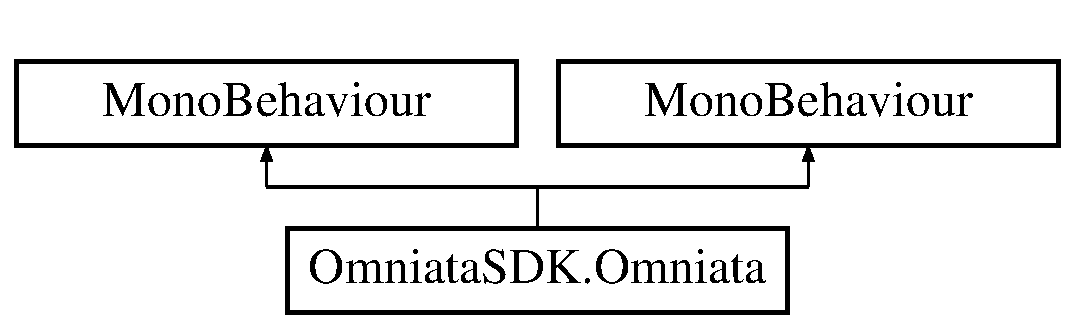
\includegraphics[height=2.000000cm]{class_omniata_s_d_k_1_1_omniata}
\end{center}
\end{figure}
\subsection*{Public Types}
\begin{DoxyCompactItemize}
\item 
enum \hyperlink{class_omniata_s_d_k_1_1_omniata_aac4ddf8e7386e787ff7ff8bab48cc6de}{Log\+Level} \{ \\*
{\bfseries Verbose} = 2, 
{\bfseries Debug}, 
{\bfseries Info}, 
{\bfseries Warn}, 
\\*
{\bfseries Error}, 
{\bfseries Assert}, 
{\bfseries Verbose} = 2, 
{\bfseries Debug}, 
\\*
{\bfseries Info}, 
{\bfseries Warn}, 
{\bfseries Error}, 
{\bfseries Assert}
 \}
\item 
enum \hyperlink{class_omniata_s_d_k_1_1_omniata_aac4ddf8e7386e787ff7ff8bab48cc6de}{Log\+Level} \{ \\*
{\bfseries Verbose} = 2, 
{\bfseries Debug}, 
{\bfseries Info}, 
{\bfseries Warn}, 
\\*
{\bfseries Error}, 
{\bfseries Assert}, 
{\bfseries Verbose} = 2, 
{\bfseries Debug}, 
\\*
{\bfseries Info}, 
{\bfseries Warn}, 
{\bfseries Error}, 
{\bfseries Assert}
 \}
\end{DoxyCompactItemize}
\subsection*{Public Member Functions}
\begin{DoxyCompactItemize}
\item 
void \hyperlink{class_omniata_s_d_k_1_1_omniata_ab14965769bf1a5b01b5b4c0089dc478f}{app\+Did\+Launch} (string A\+P\+I\+\_\+\+K\+E\+Y, string U\+I\+D, string O\+R\+G, \hyperlink{class_omniata_s_d_k_1_1_omniata_aac4ddf8e7386e787ff7ff8bab48cc6de}{Log\+Level} L\+O\+G\+L\+E\+V\+E\+L)
\begin{DoxyCompactList}\small\item\em Apps the did launch. \end{DoxyCompactList}\item 
void \hyperlink{class_omniata_s_d_k_1_1_omniata_a94fe07ba323ce0fed14b91852c7f7848}{Set\+Om\+Loglevel} (\hyperlink{class_omniata_s_d_k_1_1_omniata_aac4ddf8e7386e787ff7ff8bab48cc6de}{Log\+Level} priority)
\begin{DoxyCompactList}\small\item\em Sets the \hyperlink{class_omniata_s_d_k_1_1_omniata}{Omniata} loglevel. \end{DoxyCompactList}\item 
void \hyperlink{class_omniata_s_d_k_1_1_omniata_ab085c7c3be514851414ebe5c009f59b4}{Log\+Om} (string message)
\begin{DoxyCompactList}\small\item\em \hyperlink{class_omniata_s_d_k_1_1_omniata}{Omniata} log \end{DoxyCompactList}\item 
void \hyperlink{class_omniata_s_d_k_1_1_omniata_afebdbc87ee705a0c1e67d7a742f52f68}{Track\+Om\+Load} ()
\begin{DoxyCompactList}\small\item\em Tracks \hyperlink{class_omniata_s_d_k_1_1_omniata}{Omniata} load. \end{DoxyCompactList}\item 
void \hyperlink{class_omniata_s_d_k_1_1_omniata_a3de8b8c2d2de2000c0df1309eeac912d}{Track\+Om\+Load} (Dictionary$<$ string, string $>$ parameters)
\begin{DoxyCompactList}\small\item\em Tracks \hyperlink{class_omniata_s_d_k_1_1_omniata}{Omniata} load with parameters. \end{DoxyCompactList}\item 
void \hyperlink{class_omniata_s_d_k_1_1_omniata_a7d73aa81f2d5ba389b3af2d3cfbe6bab}{Track\+Om\+Revenue} (double total, string currency\+\_\+code)
\begin{DoxyCompactList}\small\item\em Tracks \hyperlink{class_omniata_s_d_k_1_1_omniata}{Omniata} revenue. \end{DoxyCompactList}\item 
void \hyperlink{class_omniata_s_d_k_1_1_omniata_ac187a0ef974b99a79ad7fd96792d9e14}{Track\+Om\+Revenue} (double total, string currency\+\_\+code, Dictionary$<$ string, string $>$ parameters)
\begin{DoxyCompactList}\small\item\em Tracks \hyperlink{class_omniata_s_d_k_1_1_omniata}{Omniata} revenue with parameters. \end{DoxyCompactList}\item 
void \hyperlink{class_omniata_s_d_k_1_1_omniata_af23be71f9bc730875e366452ea3866ab}{Track\+Om} (string event\+Type, Dictionary$<$ string, string $>$ parameters)
\begin{DoxyCompactList}\small\item\em Tracks \hyperlink{class_omniata_s_d_k_1_1_omniata}{Omniata} event. \end{DoxyCompactList}\item 
void \hyperlink{class_omniata_s_d_k_1_1_omniata_a3ec7dc1f37d98f16c811ce1988dd35b3}{Load\+Om\+Channel\+Message} (int channel\+I\+D)
\begin{DoxyCompactList}\small\item\em Loads \hyperlink{class_omniata_s_d_k_1_1_omniata}{Omniata} channel message. \end{DoxyCompactList}\item 
void \hyperlink{class_omniata_s_d_k_1_1_omniata_a8a8d3860177250a5c95b91a6cac07545}{Enable\+Om\+Push\+Notifications} (String device\+\_\+token)
\begin{DoxyCompactList}\small\item\em Enables \hyperlink{class_omniata_s_d_k_1_1_omniata}{Omniata} push notifications. \end{DoxyCompactList}\item 
void \hyperlink{class_omniata_s_d_k_1_1_omniata_a1c8af86696b87cbcfb9f54dcfe0ae4bd}{Disable\+Om\+Push\+Notifications} ()
\begin{DoxyCompactList}\small\item\em Disables \hyperlink{class_omniata_s_d_k_1_1_omniata}{Omniata} push notifications. \end{DoxyCompactList}\item 
void \hyperlink{class_omniata_s_d_k_1_1_omniata_ab14965769bf1a5b01b5b4c0089dc478f}{app\+Did\+Launch} (string A\+P\+I\+\_\+\+K\+E\+Y, string U\+I\+D, string O\+R\+G, \hyperlink{class_omniata_s_d_k_1_1_omniata_aac4ddf8e7386e787ff7ff8bab48cc6de}{Log\+Level} L\+O\+G\+L\+E\+V\+E\+L)
\begin{DoxyCompactList}\small\item\em Apps the did launch. \end{DoxyCompactList}\item 
void \hyperlink{class_omniata_s_d_k_1_1_omniata_a94fe07ba323ce0fed14b91852c7f7848}{Set\+Om\+Loglevel} (\hyperlink{class_omniata_s_d_k_1_1_omniata_aac4ddf8e7386e787ff7ff8bab48cc6de}{Log\+Level} priority)
\begin{DoxyCompactList}\small\item\em Sets the \hyperlink{class_omniata_s_d_k_1_1_omniata}{Omniata} loglevel. \end{DoxyCompactList}\item 
void \hyperlink{class_omniata_s_d_k_1_1_omniata_ab085c7c3be514851414ebe5c009f59b4}{Log\+Om} (string message)
\begin{DoxyCompactList}\small\item\em \hyperlink{class_omniata_s_d_k_1_1_omniata}{Omniata} log \end{DoxyCompactList}\item 
void \hyperlink{class_omniata_s_d_k_1_1_omniata_afebdbc87ee705a0c1e67d7a742f52f68}{Track\+Om\+Load} ()
\begin{DoxyCompactList}\small\item\em Tracks \hyperlink{class_omniata_s_d_k_1_1_omniata}{Omniata} load. \end{DoxyCompactList}\item 
void \hyperlink{class_omniata_s_d_k_1_1_omniata_a3de8b8c2d2de2000c0df1309eeac912d}{Track\+Om\+Load} (Dictionary$<$ string, string $>$ parameters)
\begin{DoxyCompactList}\small\item\em Tracks \hyperlink{class_omniata_s_d_k_1_1_omniata}{Omniata} load with parameters. \end{DoxyCompactList}\item 
void \hyperlink{class_omniata_s_d_k_1_1_omniata_a7d73aa81f2d5ba389b3af2d3cfbe6bab}{Track\+Om\+Revenue} (double total, string currency\+\_\+code)
\begin{DoxyCompactList}\small\item\em Tracks \hyperlink{class_omniata_s_d_k_1_1_omniata}{Omniata} revenue. \end{DoxyCompactList}\item 
void \hyperlink{class_omniata_s_d_k_1_1_omniata_ac187a0ef974b99a79ad7fd96792d9e14}{Track\+Om\+Revenue} (double total, string currency\+\_\+code, Dictionary$<$ string, string $>$ parameters)
\begin{DoxyCompactList}\small\item\em Tracks \hyperlink{class_omniata_s_d_k_1_1_omniata}{Omniata} revenue with parameters. \end{DoxyCompactList}\item 
void \hyperlink{class_omniata_s_d_k_1_1_omniata_af23be71f9bc730875e366452ea3866ab}{Track\+Om} (string event\+Type, Dictionary$<$ string, string $>$ parameters)
\begin{DoxyCompactList}\small\item\em Tracks \hyperlink{class_omniata_s_d_k_1_1_omniata}{Omniata} event. \end{DoxyCompactList}\item 
void \hyperlink{class_omniata_s_d_k_1_1_omniata_a3ec7dc1f37d98f16c811ce1988dd35b3}{Load\+Om\+Channel\+Message} (int channel\+I\+D)
\begin{DoxyCompactList}\small\item\em Loads \hyperlink{class_omniata_s_d_k_1_1_omniata}{Omniata} channel message. \end{DoxyCompactList}\item 
void \hyperlink{class_omniata_s_d_k_1_1_omniata_a8a8d3860177250a5c95b91a6cac07545}{Enable\+Om\+Push\+Notifications} (String device\+\_\+token)
\begin{DoxyCompactList}\small\item\em Enables \hyperlink{class_omniata_s_d_k_1_1_omniata}{Omniata} push notifications. \end{DoxyCompactList}\item 
void \hyperlink{class_omniata_s_d_k_1_1_omniata_a1c8af86696b87cbcfb9f54dcfe0ae4bd}{Disable\+Om\+Push\+Notifications} ()
\begin{DoxyCompactList}\small\item\em Disables \hyperlink{class_omniata_s_d_k_1_1_omniata}{Omniata} push notifications. \end{DoxyCompactList}\end{DoxyCompactItemize}
\subsection*{Public Attributes}
\begin{DoxyCompactItemize}
\item 
\hypertarget{class_omniata_s_d_k_1_1_omniata_aa3e7b8f3a3c2d478a47f7ae8a68c0cc4}{const string {\bfseries S\+D\+K\+\_\+\+V\+E\+R\+S\+I\+O\+N} = \char`\"{}unity\+S\+D\+K-\/1.\+2.\+1\char`\"{}}\label{class_omniata_s_d_k_1_1_omniata_aa3e7b8f3a3c2d478a47f7ae8a68c0cc4}

\item 
\hypertarget{class_omniata_s_d_k_1_1_omniata_a8d1a041c5bbca524be7cc5ce5c8650b6}{string {\bfseries A\+P\+I\+\_\+\+K\+E\+Y} = \char`\"{}$<$A\+P\+I K\+E\+Y$>$\char`\"{}}\label{class_omniata_s_d_k_1_1_omniata_a8d1a041c5bbca524be7cc5ce5c8650b6}

\item 
\hypertarget{class_omniata_s_d_k_1_1_omniata_a19109de42d9461cbe4a470b27c4281db}{string {\bfseries U\+I\+D} = \char`\"{}$<$User I\+D$>$\char`\"{}}\label{class_omniata_s_d_k_1_1_omniata_a19109de42d9461cbe4a470b27c4281db}

\item 
\hypertarget{class_omniata_s_d_k_1_1_omniata_a96f8e9ba7a35eeef2c7dcc4a032a58be}{string {\bfseries O\+R\+G} = \char`\"{}$<$Orgnization Name$>$\char`\"{}}\label{class_omniata_s_d_k_1_1_omniata_a96f8e9ba7a35eeef2c7dcc4a032a58be}

\item 
\hypertarget{class_omniata_s_d_k_1_1_omniata_a7c9637f0f6bc4df125fb545ab43db57b}{\hyperlink{class_omniata_s_d_k_1_1_omniata_aac4ddf8e7386e787ff7ff8bab48cc6de}{Log\+Level} {\bfseries L\+O\+G\+L\+E\+V\+E\+L} = Log\+Level.\+Verbose}\label{class_omniata_s_d_k_1_1_omniata_a7c9637f0f6bc4df125fb545ab43db57b}

\item 
\hypertarget{class_omniata_s_d_k_1_1_omniata_aee56fadb72a6796661ce45d222ecdfa8}{bool {\bfseries start\+Manually} = false}\label{class_omniata_s_d_k_1_1_omniata_aee56fadb72a6796661ce45d222ecdfa8}

\end{DoxyCompactItemize}
\subsection*{Static Public Attributes}
\begin{DoxyCompactItemize}
\item 
\hypertarget{class_omniata_s_d_k_1_1_omniata_a92be8051c963115aa7a5fb9a437f3b1e}{static string {\bfseries analyzer\+Url}}\label{class_omniata_s_d_k_1_1_omniata_a92be8051c963115aa7a5fb9a437f3b1e}

\item 
\hypertarget{class_omniata_s_d_k_1_1_omniata_a61b82ad2cf26adbe576d7fb1ebc5e492}{static string {\bfseries engager\+Url}}\label{class_omniata_s_d_k_1_1_omniata_a61b82ad2cf26adbe576d7fb1ebc5e492}

\end{DoxyCompactItemize}
\subsection*{Properties}
\begin{DoxyCompactItemize}
\item 
\hypertarget{class_omniata_s_d_k_1_1_omniata_a00e806f197055cbbb16d804cc13233b3}{static \hyperlink{class_omniata_s_d_k_1_1_omniata}{Omniata} {\bfseries Instance}\hspace{0.3cm}{\ttfamily  \mbox{[}get\mbox{]}}}\label{class_omniata_s_d_k_1_1_omniata_a00e806f197055cbbb16d804cc13233b3}

\end{DoxyCompactItemize}


\subsection{Detailed Description}
This is an Unity-\/plugin for O\+M i\+O\+S and Android S\+D\+K. Android S\+D\+K version\+: 2.\+0.\+1, i\+O\+S S\+D\+K version\+: 2.\+0.\+1 O\+M is the only integration point between a Unity application and the S\+D\+K. Details of the O\+M i\+O\+S and Android S\+D\+K, check the official documentation here\+: \href{https://omniata.atlassian.net/wiki/display/DOC/SDKs}{\tt https\+://omniata.\+atlassian.\+net/wiki/display/\+D\+O\+C/\+S\+D\+Ks} 



\subsection{Member Enumeration Documentation}
\hypertarget{class_omniata_s_d_k_1_1_omniata_aac4ddf8e7386e787ff7ff8bab48cc6de}{\index{Omniata\+S\+D\+K\+::\+Omniata@{Omniata\+S\+D\+K\+::\+Omniata}!Log\+Level@{Log\+Level}}
\index{Log\+Level@{Log\+Level}!Omniata\+S\+D\+K\+::\+Omniata@{Omniata\+S\+D\+K\+::\+Omniata}}
\subsubsection[{Log\+Level}]{\setlength{\rightskip}{0pt plus 5cm}enum {\bf Omniata\+S\+D\+K.\+Omniata.\+Log\+Level}}}\label{class_omniata_s_d_k_1_1_omniata_aac4ddf8e7386e787ff7ff8bab48cc6de}
Log\+Level value list \hypertarget{class_omniata_s_d_k_1_1_omniata_aac4ddf8e7386e787ff7ff8bab48cc6de}{\index{Omniata\+S\+D\+K\+::\+Omniata@{Omniata\+S\+D\+K\+::\+Omniata}!Log\+Level@{Log\+Level}}
\index{Log\+Level@{Log\+Level}!Omniata\+S\+D\+K\+::\+Omniata@{Omniata\+S\+D\+K\+::\+Omniata}}
\subsubsection[{Log\+Level}]{\setlength{\rightskip}{0pt plus 5cm}enum {\bf Omniata\+S\+D\+K.\+Omniata.\+Log\+Level}}}\label{class_omniata_s_d_k_1_1_omniata_aac4ddf8e7386e787ff7ff8bab48cc6de}
Log\+Level value list 

\subsection{Member Function Documentation}
\hypertarget{class_omniata_s_d_k_1_1_omniata_ab14965769bf1a5b01b5b4c0089dc478f}{\index{Omniata\+S\+D\+K\+::\+Omniata@{Omniata\+S\+D\+K\+::\+Omniata}!app\+Did\+Launch@{app\+Did\+Launch}}
\index{app\+Did\+Launch@{app\+Did\+Launch}!Omniata\+S\+D\+K\+::\+Omniata@{Omniata\+S\+D\+K\+::\+Omniata}}
\subsubsection[{app\+Did\+Launch}]{\setlength{\rightskip}{0pt plus 5cm}void Omniata\+S\+D\+K.\+Omniata.\+app\+Did\+Launch (
\begin{DoxyParamCaption}
\item[{string}]{A\+P\+I\+\_\+\+K\+E\+Y, }
\item[{string}]{U\+I\+D, }
\item[{string}]{O\+R\+G, }
\item[{{\bf Log\+Level}}]{L\+O\+G\+L\+E\+V\+E\+L}
\end{DoxyParamCaption}
)\hspace{0.3cm}{\ttfamily [inline]}}}\label{class_omniata_s_d_k_1_1_omniata_ab14965769bf1a5b01b5b4c0089dc478f}


Apps the did launch. 


\begin{DoxyParams}{Parameters}
{\em A\+P\+I\+\_\+\+K\+E\+Y} & A\+P\+I\+\_\+\+Key.\\
\hline
{\em U\+I\+D} & U\+I\+D.\\
\hline
{\em O\+R\+G} & O\+R\+G.\\
\hline
{\em L\+O\+G\+L\+E\+V\+E\+L} & L\+O\+G\+L\+E\+V\+E.\\
\hline
\end{DoxyParams}
\hypertarget{class_omniata_s_d_k_1_1_omniata_ab14965769bf1a5b01b5b4c0089dc478f}{\index{Omniata\+S\+D\+K\+::\+Omniata@{Omniata\+S\+D\+K\+::\+Omniata}!app\+Did\+Launch@{app\+Did\+Launch}}
\index{app\+Did\+Launch@{app\+Did\+Launch}!Omniata\+S\+D\+K\+::\+Omniata@{Omniata\+S\+D\+K\+::\+Omniata}}
\subsubsection[{app\+Did\+Launch}]{\setlength{\rightskip}{0pt plus 5cm}void Omniata\+S\+D\+K.\+Omniata.\+app\+Did\+Launch (
\begin{DoxyParamCaption}
\item[{string}]{A\+P\+I\+\_\+\+K\+E\+Y, }
\item[{string}]{U\+I\+D, }
\item[{string}]{O\+R\+G, }
\item[{{\bf Log\+Level}}]{L\+O\+G\+L\+E\+V\+E\+L}
\end{DoxyParamCaption}
)\hspace{0.3cm}{\ttfamily [inline]}}}\label{class_omniata_s_d_k_1_1_omniata_ab14965769bf1a5b01b5b4c0089dc478f}


Apps the did launch. 


\begin{DoxyParams}{Parameters}
{\em A\+P\+I\+\_\+\+K\+E\+Y} & A\+P\+I\+\_\+\+Key.\\
\hline
{\em U\+I\+D} & U\+I\+D.\\
\hline
{\em O\+R\+G} & O\+R\+G.\\
\hline
{\em L\+O\+G\+L\+E\+V\+E\+L} & L\+O\+G\+L\+E\+V\+E.\\
\hline
\end{DoxyParams}
\hypertarget{class_omniata_s_d_k_1_1_omniata_a1c8af86696b87cbcfb9f54dcfe0ae4bd}{\index{Omniata\+S\+D\+K\+::\+Omniata@{Omniata\+S\+D\+K\+::\+Omniata}!Disable\+Om\+Push\+Notifications@{Disable\+Om\+Push\+Notifications}}
\index{Disable\+Om\+Push\+Notifications@{Disable\+Om\+Push\+Notifications}!Omniata\+S\+D\+K\+::\+Omniata@{Omniata\+S\+D\+K\+::\+Omniata}}
\subsubsection[{Disable\+Om\+Push\+Notifications}]{\setlength{\rightskip}{0pt plus 5cm}void Omniata\+S\+D\+K.\+Omniata.\+Disable\+Om\+Push\+Notifications (
\begin{DoxyParamCaption}
{}
\end{DoxyParamCaption}
)\hspace{0.3cm}{\ttfamily [inline]}}}\label{class_omniata_s_d_k_1_1_omniata_a1c8af86696b87cbcfb9f54dcfe0ae4bd}


Disables \hyperlink{class_omniata_s_d_k_1_1_omniata}{Omniata} push notifications. 

\hypertarget{class_omniata_s_d_k_1_1_omniata_a1c8af86696b87cbcfb9f54dcfe0ae4bd}{\index{Omniata\+S\+D\+K\+::\+Omniata@{Omniata\+S\+D\+K\+::\+Omniata}!Disable\+Om\+Push\+Notifications@{Disable\+Om\+Push\+Notifications}}
\index{Disable\+Om\+Push\+Notifications@{Disable\+Om\+Push\+Notifications}!Omniata\+S\+D\+K\+::\+Omniata@{Omniata\+S\+D\+K\+::\+Omniata}}
\subsubsection[{Disable\+Om\+Push\+Notifications}]{\setlength{\rightskip}{0pt plus 5cm}void Omniata\+S\+D\+K.\+Omniata.\+Disable\+Om\+Push\+Notifications (
\begin{DoxyParamCaption}
{}
\end{DoxyParamCaption}
)\hspace{0.3cm}{\ttfamily [inline]}}}\label{class_omniata_s_d_k_1_1_omniata_a1c8af86696b87cbcfb9f54dcfe0ae4bd}


Disables \hyperlink{class_omniata_s_d_k_1_1_omniata}{Omniata} push notifications. 

\hypertarget{class_omniata_s_d_k_1_1_omniata_a8a8d3860177250a5c95b91a6cac07545}{\index{Omniata\+S\+D\+K\+::\+Omniata@{Omniata\+S\+D\+K\+::\+Omniata}!Enable\+Om\+Push\+Notifications@{Enable\+Om\+Push\+Notifications}}
\index{Enable\+Om\+Push\+Notifications@{Enable\+Om\+Push\+Notifications}!Omniata\+S\+D\+K\+::\+Omniata@{Omniata\+S\+D\+K\+::\+Omniata}}
\subsubsection[{Enable\+Om\+Push\+Notifications}]{\setlength{\rightskip}{0pt plus 5cm}void Omniata\+S\+D\+K.\+Omniata.\+Enable\+Om\+Push\+Notifications (
\begin{DoxyParamCaption}
\item[{String}]{device\+\_\+token}
\end{DoxyParamCaption}
)\hspace{0.3cm}{\ttfamily [inline]}}}\label{class_omniata_s_d_k_1_1_omniata_a8a8d3860177250a5c95b91a6cac07545}


Enables \hyperlink{class_omniata_s_d_k_1_1_omniata}{Omniata} push notifications. 


\begin{DoxyParams}{Parameters}
{\em device\+\_\+token} & Device\+\_\+token.\\
\hline
\end{DoxyParams}
\hypertarget{class_omniata_s_d_k_1_1_omniata_a8a8d3860177250a5c95b91a6cac07545}{\index{Omniata\+S\+D\+K\+::\+Omniata@{Omniata\+S\+D\+K\+::\+Omniata}!Enable\+Om\+Push\+Notifications@{Enable\+Om\+Push\+Notifications}}
\index{Enable\+Om\+Push\+Notifications@{Enable\+Om\+Push\+Notifications}!Omniata\+S\+D\+K\+::\+Omniata@{Omniata\+S\+D\+K\+::\+Omniata}}
\subsubsection[{Enable\+Om\+Push\+Notifications}]{\setlength{\rightskip}{0pt plus 5cm}void Omniata\+S\+D\+K.\+Omniata.\+Enable\+Om\+Push\+Notifications (
\begin{DoxyParamCaption}
\item[{String}]{device\+\_\+token}
\end{DoxyParamCaption}
)\hspace{0.3cm}{\ttfamily [inline]}}}\label{class_omniata_s_d_k_1_1_omniata_a8a8d3860177250a5c95b91a6cac07545}


Enables \hyperlink{class_omniata_s_d_k_1_1_omniata}{Omniata} push notifications. 


\begin{DoxyParams}{Parameters}
{\em device\+\_\+token} & Device\+\_\+token.\\
\hline
\end{DoxyParams}
\hypertarget{class_omniata_s_d_k_1_1_omniata_a3ec7dc1f37d98f16c811ce1988dd35b3}{\index{Omniata\+S\+D\+K\+::\+Omniata@{Omniata\+S\+D\+K\+::\+Omniata}!Load\+Om\+Channel\+Message@{Load\+Om\+Channel\+Message}}
\index{Load\+Om\+Channel\+Message@{Load\+Om\+Channel\+Message}!Omniata\+S\+D\+K\+::\+Omniata@{Omniata\+S\+D\+K\+::\+Omniata}}
\subsubsection[{Load\+Om\+Channel\+Message}]{\setlength{\rightskip}{0pt plus 5cm}void Omniata\+S\+D\+K.\+Omniata.\+Load\+Om\+Channel\+Message (
\begin{DoxyParamCaption}
\item[{int}]{channel\+I\+D}
\end{DoxyParamCaption}
)\hspace{0.3cm}{\ttfamily [inline]}}}\label{class_omniata_s_d_k_1_1_omniata_a3ec7dc1f37d98f16c811ce1988dd35b3}


Loads \hyperlink{class_omniata_s_d_k_1_1_omniata}{Omniata} channel message. 


\begin{DoxyParams}{Parameters}
{\em channel\+I\+D} & Channel I\+D.\\
\hline
\end{DoxyParams}
\hypertarget{class_omniata_s_d_k_1_1_omniata_a3ec7dc1f37d98f16c811ce1988dd35b3}{\index{Omniata\+S\+D\+K\+::\+Omniata@{Omniata\+S\+D\+K\+::\+Omniata}!Load\+Om\+Channel\+Message@{Load\+Om\+Channel\+Message}}
\index{Load\+Om\+Channel\+Message@{Load\+Om\+Channel\+Message}!Omniata\+S\+D\+K\+::\+Omniata@{Omniata\+S\+D\+K\+::\+Omniata}}
\subsubsection[{Load\+Om\+Channel\+Message}]{\setlength{\rightskip}{0pt plus 5cm}void Omniata\+S\+D\+K.\+Omniata.\+Load\+Om\+Channel\+Message (
\begin{DoxyParamCaption}
\item[{int}]{channel\+I\+D}
\end{DoxyParamCaption}
)\hspace{0.3cm}{\ttfamily [inline]}}}\label{class_omniata_s_d_k_1_1_omniata_a3ec7dc1f37d98f16c811ce1988dd35b3}


Loads \hyperlink{class_omniata_s_d_k_1_1_omniata}{Omniata} channel message. 


\begin{DoxyParams}{Parameters}
{\em channel\+I\+D} & Channel I\+D.\\
\hline
\end{DoxyParams}
\hypertarget{class_omniata_s_d_k_1_1_omniata_ab085c7c3be514851414ebe5c009f59b4}{\index{Omniata\+S\+D\+K\+::\+Omniata@{Omniata\+S\+D\+K\+::\+Omniata}!Log\+Om@{Log\+Om}}
\index{Log\+Om@{Log\+Om}!Omniata\+S\+D\+K\+::\+Omniata@{Omniata\+S\+D\+K\+::\+Omniata}}
\subsubsection[{Log\+Om}]{\setlength{\rightskip}{0pt plus 5cm}void Omniata\+S\+D\+K.\+Omniata.\+Log\+Om (
\begin{DoxyParamCaption}
\item[{string}]{message}
\end{DoxyParamCaption}
)\hspace{0.3cm}{\ttfamily [inline]}}}\label{class_omniata_s_d_k_1_1_omniata_ab085c7c3be514851414ebe5c009f59b4}


\hyperlink{class_omniata_s_d_k_1_1_omniata}{Omniata} log 


\begin{DoxyParams}{Parameters}
{\em message} & Message.\\
\hline
\end{DoxyParams}
\hypertarget{class_omniata_s_d_k_1_1_omniata_ab085c7c3be514851414ebe5c009f59b4}{\index{Omniata\+S\+D\+K\+::\+Omniata@{Omniata\+S\+D\+K\+::\+Omniata}!Log\+Om@{Log\+Om}}
\index{Log\+Om@{Log\+Om}!Omniata\+S\+D\+K\+::\+Omniata@{Omniata\+S\+D\+K\+::\+Omniata}}
\subsubsection[{Log\+Om}]{\setlength{\rightskip}{0pt plus 5cm}void Omniata\+S\+D\+K.\+Omniata.\+Log\+Om (
\begin{DoxyParamCaption}
\item[{string}]{message}
\end{DoxyParamCaption}
)\hspace{0.3cm}{\ttfamily [inline]}}}\label{class_omniata_s_d_k_1_1_omniata_ab085c7c3be514851414ebe5c009f59b4}


\hyperlink{class_omniata_s_d_k_1_1_omniata}{Omniata} log 


\begin{DoxyParams}{Parameters}
{\em message} & Message.\\
\hline
\end{DoxyParams}
\hypertarget{class_omniata_s_d_k_1_1_omniata_a94fe07ba323ce0fed14b91852c7f7848}{\index{Omniata\+S\+D\+K\+::\+Omniata@{Omniata\+S\+D\+K\+::\+Omniata}!Set\+Om\+Loglevel@{Set\+Om\+Loglevel}}
\index{Set\+Om\+Loglevel@{Set\+Om\+Loglevel}!Omniata\+S\+D\+K\+::\+Omniata@{Omniata\+S\+D\+K\+::\+Omniata}}
\subsubsection[{Set\+Om\+Loglevel}]{\setlength{\rightskip}{0pt plus 5cm}void Omniata\+S\+D\+K.\+Omniata.\+Set\+Om\+Loglevel (
\begin{DoxyParamCaption}
\item[{{\bf Log\+Level}}]{priority}
\end{DoxyParamCaption}
)\hspace{0.3cm}{\ttfamily [inline]}}}\label{class_omniata_s_d_k_1_1_omniata_a94fe07ba323ce0fed14b91852c7f7848}


Sets the \hyperlink{class_omniata_s_d_k_1_1_omniata}{Omniata} loglevel. 


\begin{DoxyParams}{Parameters}
{\em priority} & the priority of the loglevel\\
\hline
\end{DoxyParams}
\hypertarget{class_omniata_s_d_k_1_1_omniata_a94fe07ba323ce0fed14b91852c7f7848}{\index{Omniata\+S\+D\+K\+::\+Omniata@{Omniata\+S\+D\+K\+::\+Omniata}!Set\+Om\+Loglevel@{Set\+Om\+Loglevel}}
\index{Set\+Om\+Loglevel@{Set\+Om\+Loglevel}!Omniata\+S\+D\+K\+::\+Omniata@{Omniata\+S\+D\+K\+::\+Omniata}}
\subsubsection[{Set\+Om\+Loglevel}]{\setlength{\rightskip}{0pt plus 5cm}void Omniata\+S\+D\+K.\+Omniata.\+Set\+Om\+Loglevel (
\begin{DoxyParamCaption}
\item[{{\bf Log\+Level}}]{priority}
\end{DoxyParamCaption}
)\hspace{0.3cm}{\ttfamily [inline]}}}\label{class_omniata_s_d_k_1_1_omniata_a94fe07ba323ce0fed14b91852c7f7848}


Sets the \hyperlink{class_omniata_s_d_k_1_1_omniata}{Omniata} loglevel. 


\begin{DoxyParams}{Parameters}
{\em priority} & the priority of the loglevel\\
\hline
\end{DoxyParams}
\hypertarget{class_omniata_s_d_k_1_1_omniata_af23be71f9bc730875e366452ea3866ab}{\index{Omniata\+S\+D\+K\+::\+Omniata@{Omniata\+S\+D\+K\+::\+Omniata}!Track\+Om@{Track\+Om}}
\index{Track\+Om@{Track\+Om}!Omniata\+S\+D\+K\+::\+Omniata@{Omniata\+S\+D\+K\+::\+Omniata}}
\subsubsection[{Track\+Om}]{\setlength{\rightskip}{0pt plus 5cm}void Omniata\+S\+D\+K.\+Omniata.\+Track\+Om (
\begin{DoxyParamCaption}
\item[{string}]{event\+Type, }
\item[{Dictionary$<$ string, string $>$}]{parameters}
\end{DoxyParamCaption}
)\hspace{0.3cm}{\ttfamily [inline]}}}\label{class_omniata_s_d_k_1_1_omniata_af23be71f9bc730875e366452ea3866ab}


Tracks \hyperlink{class_omniata_s_d_k_1_1_omniata}{Omniata} event. 


\begin{DoxyParams}{Parameters}
{\em event\+Type} & Event type.\\
\hline
{\em parameters} & Parameters.\\
\hline
\end{DoxyParams}
\hypertarget{class_omniata_s_d_k_1_1_omniata_af23be71f9bc730875e366452ea3866ab}{\index{Omniata\+S\+D\+K\+::\+Omniata@{Omniata\+S\+D\+K\+::\+Omniata}!Track\+Om@{Track\+Om}}
\index{Track\+Om@{Track\+Om}!Omniata\+S\+D\+K\+::\+Omniata@{Omniata\+S\+D\+K\+::\+Omniata}}
\subsubsection[{Track\+Om}]{\setlength{\rightskip}{0pt plus 5cm}void Omniata\+S\+D\+K.\+Omniata.\+Track\+Om (
\begin{DoxyParamCaption}
\item[{string}]{event\+Type, }
\item[{Dictionary$<$ string, string $>$}]{parameters}
\end{DoxyParamCaption}
)\hspace{0.3cm}{\ttfamily [inline]}}}\label{class_omniata_s_d_k_1_1_omniata_af23be71f9bc730875e366452ea3866ab}


Tracks \hyperlink{class_omniata_s_d_k_1_1_omniata}{Omniata} event. 


\begin{DoxyParams}{Parameters}
{\em event\+Type} & Event type.\\
\hline
{\em parameters} & Parameters.\\
\hline
\end{DoxyParams}
\hypertarget{class_omniata_s_d_k_1_1_omniata_afebdbc87ee705a0c1e67d7a742f52f68}{\index{Omniata\+S\+D\+K\+::\+Omniata@{Omniata\+S\+D\+K\+::\+Omniata}!Track\+Om\+Load@{Track\+Om\+Load}}
\index{Track\+Om\+Load@{Track\+Om\+Load}!Omniata\+S\+D\+K\+::\+Omniata@{Omniata\+S\+D\+K\+::\+Omniata}}
\subsubsection[{Track\+Om\+Load}]{\setlength{\rightskip}{0pt plus 5cm}void Omniata\+S\+D\+K.\+Omniata.\+Track\+Om\+Load (
\begin{DoxyParamCaption}
{}
\end{DoxyParamCaption}
)\hspace{0.3cm}{\ttfamily [inline]}}}\label{class_omniata_s_d_k_1_1_omniata_afebdbc87ee705a0c1e67d7a742f52f68}


Tracks \hyperlink{class_omniata_s_d_k_1_1_omniata}{Omniata} load. 

\hypertarget{class_omniata_s_d_k_1_1_omniata_afebdbc87ee705a0c1e67d7a742f52f68}{\index{Omniata\+S\+D\+K\+::\+Omniata@{Omniata\+S\+D\+K\+::\+Omniata}!Track\+Om\+Load@{Track\+Om\+Load}}
\index{Track\+Om\+Load@{Track\+Om\+Load}!Omniata\+S\+D\+K\+::\+Omniata@{Omniata\+S\+D\+K\+::\+Omniata}}
\subsubsection[{Track\+Om\+Load}]{\setlength{\rightskip}{0pt plus 5cm}void Omniata\+S\+D\+K.\+Omniata.\+Track\+Om\+Load (
\begin{DoxyParamCaption}
{}
\end{DoxyParamCaption}
)\hspace{0.3cm}{\ttfamily [inline]}}}\label{class_omniata_s_d_k_1_1_omniata_afebdbc87ee705a0c1e67d7a742f52f68}


Tracks \hyperlink{class_omniata_s_d_k_1_1_omniata}{Omniata} load. 

\hypertarget{class_omniata_s_d_k_1_1_omniata_a3de8b8c2d2de2000c0df1309eeac912d}{\index{Omniata\+S\+D\+K\+::\+Omniata@{Omniata\+S\+D\+K\+::\+Omniata}!Track\+Om\+Load@{Track\+Om\+Load}}
\index{Track\+Om\+Load@{Track\+Om\+Load}!Omniata\+S\+D\+K\+::\+Omniata@{Omniata\+S\+D\+K\+::\+Omniata}}
\subsubsection[{Track\+Om\+Load}]{\setlength{\rightskip}{0pt plus 5cm}void Omniata\+S\+D\+K.\+Omniata.\+Track\+Om\+Load (
\begin{DoxyParamCaption}
\item[{Dictionary$<$ string, string $>$}]{parameters}
\end{DoxyParamCaption}
)\hspace{0.3cm}{\ttfamily [inline]}}}\label{class_omniata_s_d_k_1_1_omniata_a3de8b8c2d2de2000c0df1309eeac912d}


Tracks \hyperlink{class_omniata_s_d_k_1_1_omniata}{Omniata} load with parameters. 


\begin{DoxyParams}{Parameters}
{\em parameters} & Parameters.\\
\hline
\end{DoxyParams}
\hypertarget{class_omniata_s_d_k_1_1_omniata_a3de8b8c2d2de2000c0df1309eeac912d}{\index{Omniata\+S\+D\+K\+::\+Omniata@{Omniata\+S\+D\+K\+::\+Omniata}!Track\+Om\+Load@{Track\+Om\+Load}}
\index{Track\+Om\+Load@{Track\+Om\+Load}!Omniata\+S\+D\+K\+::\+Omniata@{Omniata\+S\+D\+K\+::\+Omniata}}
\subsubsection[{Track\+Om\+Load}]{\setlength{\rightskip}{0pt plus 5cm}void Omniata\+S\+D\+K.\+Omniata.\+Track\+Om\+Load (
\begin{DoxyParamCaption}
\item[{Dictionary$<$ string, string $>$}]{parameters}
\end{DoxyParamCaption}
)\hspace{0.3cm}{\ttfamily [inline]}}}\label{class_omniata_s_d_k_1_1_omniata_a3de8b8c2d2de2000c0df1309eeac912d}


Tracks \hyperlink{class_omniata_s_d_k_1_1_omniata}{Omniata} load with parameters. 


\begin{DoxyParams}{Parameters}
{\em parameters} & Parameters.\\
\hline
\end{DoxyParams}
\hypertarget{class_omniata_s_d_k_1_1_omniata_a7d73aa81f2d5ba389b3af2d3cfbe6bab}{\index{Omniata\+S\+D\+K\+::\+Omniata@{Omniata\+S\+D\+K\+::\+Omniata}!Track\+Om\+Revenue@{Track\+Om\+Revenue}}
\index{Track\+Om\+Revenue@{Track\+Om\+Revenue}!Omniata\+S\+D\+K\+::\+Omniata@{Omniata\+S\+D\+K\+::\+Omniata}}
\subsubsection[{Track\+Om\+Revenue}]{\setlength{\rightskip}{0pt plus 5cm}void Omniata\+S\+D\+K.\+Omniata.\+Track\+Om\+Revenue (
\begin{DoxyParamCaption}
\item[{double}]{total, }
\item[{string}]{currency\+\_\+code}
\end{DoxyParamCaption}
)\hspace{0.3cm}{\ttfamily [inline]}}}\label{class_omniata_s_d_k_1_1_omniata_a7d73aa81f2d5ba389b3af2d3cfbe6bab}


Tracks \hyperlink{class_omniata_s_d_k_1_1_omniata}{Omniata} revenue. 


\begin{DoxyParams}{Parameters}
{\em total} & Total.\\
\hline
{\em currency\+\_\+code} & Currency\+\_\+code.\\
\hline
\end{DoxyParams}
\hypertarget{class_omniata_s_d_k_1_1_omniata_a7d73aa81f2d5ba389b3af2d3cfbe6bab}{\index{Omniata\+S\+D\+K\+::\+Omniata@{Omniata\+S\+D\+K\+::\+Omniata}!Track\+Om\+Revenue@{Track\+Om\+Revenue}}
\index{Track\+Om\+Revenue@{Track\+Om\+Revenue}!Omniata\+S\+D\+K\+::\+Omniata@{Omniata\+S\+D\+K\+::\+Omniata}}
\subsubsection[{Track\+Om\+Revenue}]{\setlength{\rightskip}{0pt plus 5cm}void Omniata\+S\+D\+K.\+Omniata.\+Track\+Om\+Revenue (
\begin{DoxyParamCaption}
\item[{double}]{total, }
\item[{string}]{currency\+\_\+code}
\end{DoxyParamCaption}
)\hspace{0.3cm}{\ttfamily [inline]}}}\label{class_omniata_s_d_k_1_1_omniata_a7d73aa81f2d5ba389b3af2d3cfbe6bab}


Tracks \hyperlink{class_omniata_s_d_k_1_1_omniata}{Omniata} revenue. 


\begin{DoxyParams}{Parameters}
{\em total} & Total.\\
\hline
{\em currency\+\_\+code} & Currency\+\_\+code.\\
\hline
\end{DoxyParams}
\hypertarget{class_omniata_s_d_k_1_1_omniata_ac187a0ef974b99a79ad7fd96792d9e14}{\index{Omniata\+S\+D\+K\+::\+Omniata@{Omniata\+S\+D\+K\+::\+Omniata}!Track\+Om\+Revenue@{Track\+Om\+Revenue}}
\index{Track\+Om\+Revenue@{Track\+Om\+Revenue}!Omniata\+S\+D\+K\+::\+Omniata@{Omniata\+S\+D\+K\+::\+Omniata}}
\subsubsection[{Track\+Om\+Revenue}]{\setlength{\rightskip}{0pt plus 5cm}void Omniata\+S\+D\+K.\+Omniata.\+Track\+Om\+Revenue (
\begin{DoxyParamCaption}
\item[{double}]{total, }
\item[{string}]{currency\+\_\+code, }
\item[{Dictionary$<$ string, string $>$}]{parameters}
\end{DoxyParamCaption}
)\hspace{0.3cm}{\ttfamily [inline]}}}\label{class_omniata_s_d_k_1_1_omniata_ac187a0ef974b99a79ad7fd96792d9e14}


Tracks \hyperlink{class_omniata_s_d_k_1_1_omniata}{Omniata} revenue with parameters. 


\begin{DoxyParams}{Parameters}
{\em total} & Total.\\
\hline
{\em currency\+\_\+code} & Currency\+\_\+code.\\
\hline
{\em parameters} & Parameters.\\
\hline
\end{DoxyParams}
\hypertarget{class_omniata_s_d_k_1_1_omniata_ac187a0ef974b99a79ad7fd96792d9e14}{\index{Omniata\+S\+D\+K\+::\+Omniata@{Omniata\+S\+D\+K\+::\+Omniata}!Track\+Om\+Revenue@{Track\+Om\+Revenue}}
\index{Track\+Om\+Revenue@{Track\+Om\+Revenue}!Omniata\+S\+D\+K\+::\+Omniata@{Omniata\+S\+D\+K\+::\+Omniata}}
\subsubsection[{Track\+Om\+Revenue}]{\setlength{\rightskip}{0pt plus 5cm}void Omniata\+S\+D\+K.\+Omniata.\+Track\+Om\+Revenue (
\begin{DoxyParamCaption}
\item[{double}]{total, }
\item[{string}]{currency\+\_\+code, }
\item[{Dictionary$<$ string, string $>$}]{parameters}
\end{DoxyParamCaption}
)\hspace{0.3cm}{\ttfamily [inline]}}}\label{class_omniata_s_d_k_1_1_omniata_ac187a0ef974b99a79ad7fd96792d9e14}


Tracks \hyperlink{class_omniata_s_d_k_1_1_omniata}{Omniata} revenue with parameters. 


\begin{DoxyParams}{Parameters}
{\em total} & Total.\\
\hline
{\em currency\+\_\+code} & Currency\+\_\+code.\\
\hline
{\em parameters} & Parameters.\\
\hline
\end{DoxyParams}


The documentation for this class was generated from the following file\+:\begin{DoxyCompactItemize}
\item 
Omniata.\+cs\end{DoxyCompactItemize}

%--- End generated contents ---

% Index
\newpage
\phantomsection
\addcontentsline{toc}{chapter}{Index}
\printindex

\end{document}
